%
% transpositionen.tex -- Permutationen aus Transpositionen erzeugen
%
% (c) 2020 Prof Dr Andreas Müller, Hochschule Rapperswil
%
\section{Permutationen und Transpositionen
\label{buch:section:permutationen-und-transpositionen}}
\rhead{Transpositionen}
Im vorangegangenen Abschnitt haben wir Permutationen durch die
Zyklenzerlegung charakterisiert.
Es zeigt sich aber, dass sich eine Permutation in noch elementarere
Bausteine zerlegen lässt, die Transpositionen.

\begin{definition}
Einen Transposition $\tau\in S_n$ ist ein Permutation, die genau
zwei Elemente vertauscht.
Die Transposition $\tau_{ij}$ ist definiert durch
\[
\tau_{ij}(x)
=
\begin{cases}
i&\qquad x=j\\
j&\qquad x=i\\
x&\qquad\text{sonst.}
\end{cases}
\]
\end{definition}

Eine Transposition hat genau einen Zyklus der Länge $2$, alle anderen
Zyklen haben die Länge $1$.

\subsection{Zyklus und Permutationen aus Transpositionen}
Sei $\sigma$ die zyklische Vertauschung der Elemente $1,\dots,k\in [n]$,
also die Permutation, die $1\to2\to3\to\dots\to k-2\to k-1\to k\to 1$
abbildet.
Dieser Zyklus lässt sich wie folgt aus Transpositionen zusammensetzen:
\begin{center}
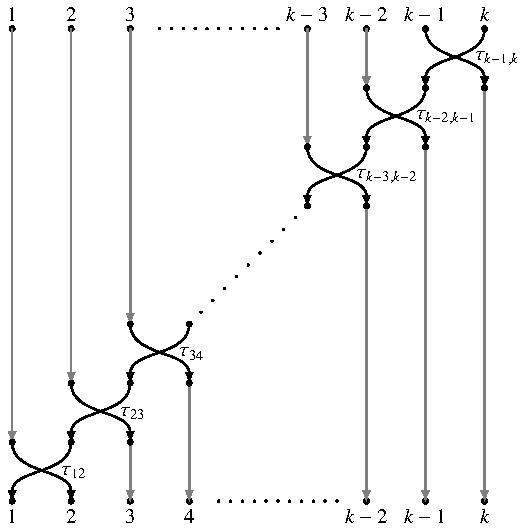
\includegraphics{chapters/50-permutationen/images/transpositionen.pdf}
\end{center}
Es ist also
\[
\sigma 
=
\tau_{12} \tau_{23} \tau_{34} \dots \tau_{k-3,k-2} \tau_{k-2,k-1} \tau_{k-1,k}.
\]
\begin{satz}
Jede Permutation $\sigma\in S_n$ lässt sich als ein Produkt von 
Transpositionen schreiben.
Jeder Zyklus der Länge $k$ lässt sich aus $k-1$ Transpositionen
zusammensetzen.
Eine Permutation mit einer Zerlegung in Zyklen der Längen $l_1,\dots,l_p$
kann als Produkt von $l_1+\dots+l_p-p$ Transpositionen geschrieben werden.
\end{satz}

\subsection{Signum einer Permutation}
Die Anzahl Transpositionen, die benötigt werden, um eine Permutation
zu beschreiben, ist nicht fest. 
Wenn $\sigma$ mit $k$ Transpositionen geschrieben werden kann und
$\gamma$ mit $l$, dann hat $\gamma\sigma\gamma^{-1}$ die gleiche
Zyklenzerlegung, kann aber mit $k+2l$ Transpositionen geschrieben
werden.
Die Anzahl Transpositionen, die zur Darstellung einer Permutation
nötig ist, ändert sich aber immer nur um eine gerade Zahl.
Die Anzahl ist also keine Invariante einer Permutation, aber ob
die Anzahl gerade ist oder nicht, ist sehr wohl eine charkterisierende
Eigenschaft einer Permutation.

\begin{definition}
Das {\em Vorzeichen} oder {\em Signum} einer Permutation $\sigma$ ist
die Zahl $\operatorname{sgn}(\sigma)=(-1)^k$, wenn $\sigma$ als Produkt
von $k$ Transpositionen geschrieben werden kann.
\end{definition}

Die inverse Permutation $\sigma^{-1}$ hat das gleiche Signum wie $\sigma$.
Wenn nämlich $\sigma= \tau_1\tau_2\dots\tau_k$ geschrieben werden kann,
dann ist $\sigma^{-1}=\tau_k\dots\tau_2\tau_1$, sowohl $\sigma$ wie
$\sigma^{-1}$ können also mit der gleichen Zahl von Transpositionen
geschrieben werden, sie haben also auch das gleiche Vorzeichen.

Die Abbildung $S_n\to\{\pm\}$, die einer Permutation das Signum zuordnet,
ist ein Homomorphismus von Gruppen,
d.~h.
\[
\operatorname{sgn}(\sigma_1\sigma_2)
=
\operatorname{sgn}(\sigma_1)
\operatorname{sgn}(\sigma_2)
\]
da ganz offensichtlich $\sigma_1\sigma_2$ mit $k_1+k_2$ Transpositionen
geschrieben kann, wenn $\sigma_i$ mit $k_i$ Transpositionen geschrieben
werden kann.

Das Signum definiert in der symmetrischen Gruppe eine Teilmenge bestehnd
aus den Permutationen mit Signum $+1$.

\begin{definition}
Die Teilmenge
\[
A_n
=
\{
\sigma\in S_n\;|\; \operatorname{sgn}(\sigma)=1
\}
\subset S_n.
\]
heisst die {\em alternierende Gruppe} der Ordnung $n$
Die Elemente von $A_n$ heissen auch die {\em geraden} Permutationen,
die
Elemente von $S_n\setminus A_n$ heissen auch die {\em ungeraden}
Permutationen.
\end{definition}

Die alternierende Gruppe $A_n$ ist tatsächlich eine Untergruppe.
Zunächst ist $\operatorname{sgn}(e)=(-1)^0=1$, also ist $e\in A_n$.
Es wurde schon gezeigt, dass mit jedem Element $\sigma\in A_n$ auch
das inverse Element $\sigma^{-1}\in A_n$ ist.
Es muss aber noch sichergestellt werden, dass das Produkt von zwei
geraden Transpositionen wieder gerade ist:
\[
\begin{aligned}
\sigma_1,\sigma_2&\in A_n
&\Rightarrow&&
\operatorname{sgn}(\sigma_1)
&=
\operatorname{sgn}(\sigma_2)
=
1
\\
&&\Rightarrow&&
\operatorname{sgn}(\sigma_1\sigma_2)
&=
\operatorname{sgn}(\sigma_1)
\operatorname{sgn}(\sigma_2)
=
1\cdot 1=1
&&\Rightarrow&
\sigma_1\sigma_2&\in A_n.
\end{aligned}
\]
Damit ist gezeigt, dass die alternierende Gruppe $A_n$ ein Untergruppe von 
$S_n$ ist.

